\documentclass[11pt,a4paper]{article}
\usepackage[margin=1in]{geometry}
\usepackage{amsmath}
\usepackage{booktabs}
\usepackage{graphicx}
\usepackage{siunitx}

\title{PY2105 --- Assignment 4 Report}
\author{}
\date{}

\begin{document}
\maketitle

\section{Linear systems}
The system was solved using Gaussian elimination with partial pivoting and an
unpivoted LU factorisation, with forward and backward substitution. No
preconstructed matrix solver was used.

The upper-triangular matrix and transformed right-hand side after Gaussian
elimination with partial pivoting were
\[
U_{\mathrm{G}}=
\begin{bmatrix}
13&4&7&9\\
0&13.076923&13.384615&8.923077\\
0&0&-6.411765&10.058824\\
0&0&0&-2.214679
\end{bmatrix},\qquad
b_{\mathrm{G}}=
\begin{bmatrix}
111\\137.384615\\24.647059\\-11.073395
\end{bmatrix}.
\]
Back substitution gives
\[
x=\begin{bmatrix}2&3&4&5\end{bmatrix}^{T},
\qquad \det(A)=-2414.
\]

The LU factorisation, satisfying \(A=LU\), is
\[
\begin{aligned}
L&=
\begin{bmatrix}
1&0&0&0\\
0.769231&1&0&0\\
0.076923&2.631579&1&0\\
0.230769&4.473684&6.106383&1
\end{bmatrix},\\[1ex]
U&=
\begin{bmatrix}
13&4&7&9\\
0&2.923077&-0.384615&5.076923\\
0&0&2.473684&1.947368\\
0&0&0&-25.680851
\end{bmatrix}.
\end{aligned}
\]
Solving \(Ly=b\) and then \(Ux=y\) gives the same solution. The inverse,
computed by solving \(A z=e_j\) for each column \(e_j\), is
\[
A^{-1}\approx
\begin{bmatrix}
-0.197183&0.376139&-0.163215&-0.011599\\
-0.781690&1.033140&-0.384424&0.071665\\
0.521127&-0.708368&0.217067&0.030655\\
0.338028&-0.451533&0.237780&-0.038940
\end{bmatrix}.
\]

\section{Monte Carlo estimate of \(\pi\)}
Uniform points were sampled in a square of side \(a=2\), centred at the
origin. The circle has radius \(a/2=1\). If \(N_c\) of \(N_s\) points fall
inside the circle, the estimate is
\[
\widehat{\pi}=4\frac{N_c}{N_s}.
\]
For \(10{,}000{,}000\) points, the result was
\(\widehat{\pi}=3.1419404\), with relative error \(0.0110691\%\). The
precision plot shows the measured relative error at increasing sample
counts. Monte Carlo error is expected to scale statistically as
\(N^{-1/2}\); an individual run need not decrease monotonically, as seen in
the plot.

\begin{figure}[htbp]
  \centering
  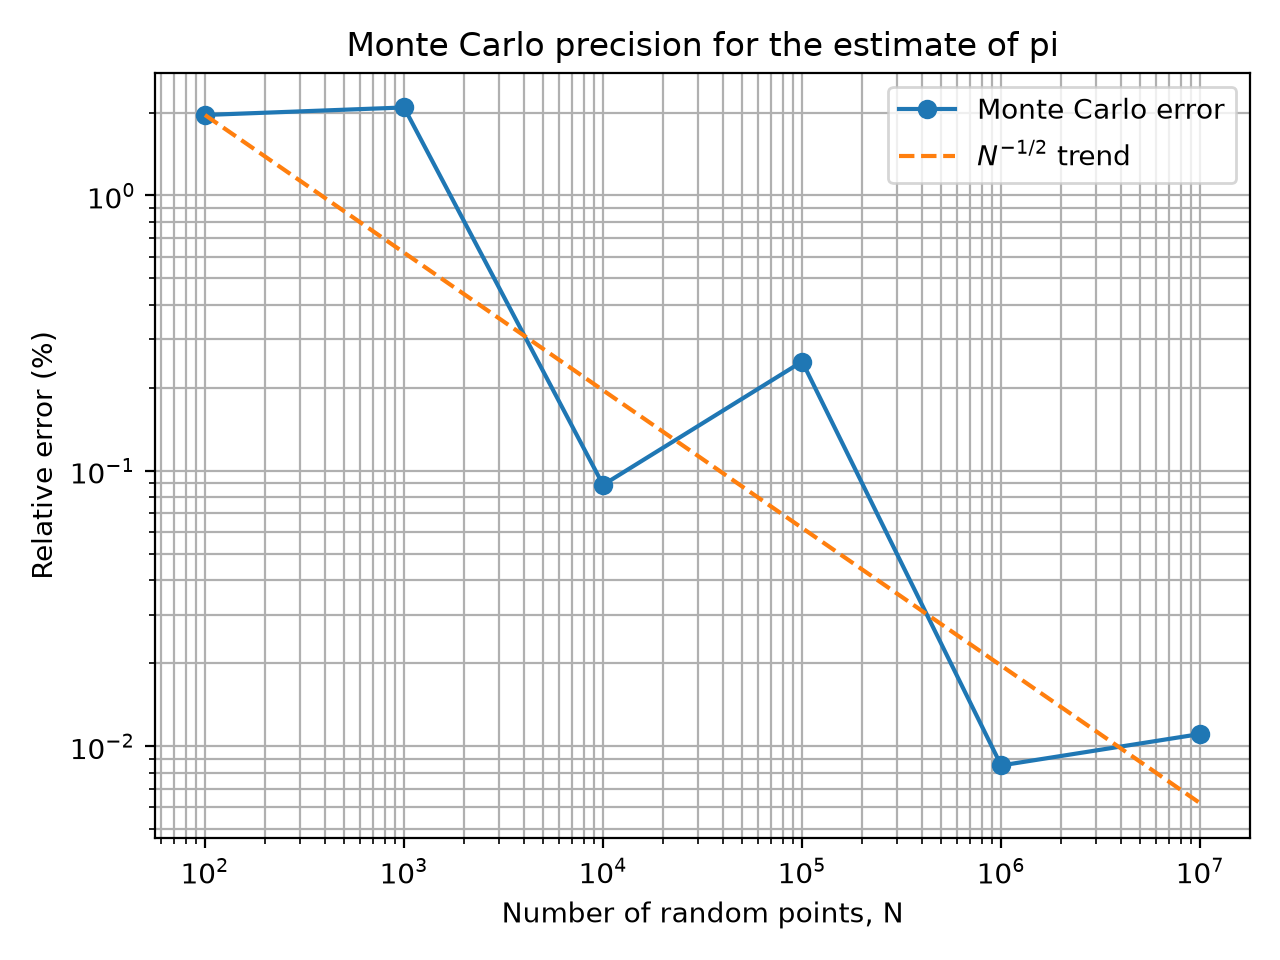
\includegraphics[width=0.88\textwidth]{pi_precision.png}
  \caption{Relative error in the Monte Carlo estimate of \(\pi\) versus
  sample count. The dashed line shows an \(N^{-1/2}\) reference trend.}
  \label{fig:pi-precision}
\end{figure}

\section{Monte Carlo integration}
The integrand is
\[
f(x)=\frac{300x}{1+e^x},\qquad 0\leq x\leq 10.
\]
The bounding rectangle used for hit-or-miss sampling was
\([0,10]\times[0,100]\). It encloses the function throughout the interval.
The numerical reference integral, evaluated using the trapezoidal rule with
one million intervals, was \(246.5902935\).

Using the binomial standard error to estimate a sample count for a
\(0.01\%\) relative error at approximately \(95\%\) confidence gave
\(1{,}173{,}727{,}761\) Monte Carlo points. One run returned
\(246.5882359\), a relative error of \(0.0008344\%\) against the reference.
The measured time was \(248.04\) s.

The trapezoidal rule required 226 intervals (step size
\(h=10/226\approx0.0442478\)) to obtain a relative error below \(0.01\%\)
against the same reference. Its result was \(246.5658002\), with relative
error \(0.0099328\%\), and measured runtime \(0.0000884\) s. In this run,
the Monte Carlo calculation took about \(2.8\times10^6\) times longer.
Runtime depends on the machine and measurement conditions; the main
computational difference is that the Monte Carlo estimate required over a
billion samples.

\end{document}
